\documentclass[10pt, a4paper]{book}
\usepackage[spanish]{babel}
\usepackage[utf8]{inputenc}
\usepackage{xparse}
\usepackage{multirow}
%%Tipografia
\usepackage{newpxtext} \usepackage[euler-digits]{eulervm}
%%
\usepackage{listings}
\usepackage[margin=1in]{geometry} 
\usepackage{amsmath,amsthm,amssymb}
\usepackage{booktabs}
\usepackage[table,xcdraw]{xcolor}
\usepackage{tikz}
\usepackage{esvect}
\usepackage{tcolorbox}
\usetikzlibrary{arrows,positioning,fit,shapes,calc}
\usepackage{framed}
\usepackage{fancyhdr} 
\usepackage[
    type={CC},
    modifier={by-nc},
    version={4.0},
]{doclicense}
\pagestyle{fancy} 
\usepackage{chessboard}
\storechessboardstyle{5x5}{maxfield=e5}
\fancyhead[RE,RO]{\nouppercase{\leftmark}}
\fancyhead[LE,LO]{\nouppercase{\rightmark}}

\usetikzlibrary{calc,angles,positioning,intersections,quotes,decorations.markings}
\usepackage{tkz-euclide}
\usetkzobj{all}
\usepackage{pgfplots}
\usepackage{graphicx}
\usepackage{subfigure}
\usepackage{float}
\usepackage{multicol}
\usepackage{color}
 
\definecolor{codegreen}{rgb}{0,0.6,0}
\definecolor{codegray}{rgb}{0.5,0.5,0.5}
\definecolor{codepurple}{rgb}{0.58,0,0.82}
\definecolor{backcolour}{rgb}{0.95,0.95,0.92}
 
\lstdefinestyle{mystyle}{
    backgroundcolor=\color{backcolour},   
    commentstyle=\color{codegreen},
    keywordstyle=\color{magenta},
    numberstyle=\tiny\color{codegray},
    stringstyle=\color{codepurple},
    basicstyle=\footnotesize,
    breakatwhitespace=false,         
    breaklines=true,                 
    captionpos=b,                    
    keepspaces=true,                 
    numbers=left,                    
    numbersep=5pt,                  
    showspaces=false,                
    showstringspaces=false,
    showtabs=false,                  
    tabsize=2
}
 
\lstset{style=mystyle}
\pgfplotsset{compat=1.5}

%%%%%%%%%%%%%%%%%%%%% Dibujar funciones 
% https://es.sharelatex.com/learn/Pgfplots_package
% http://pgfplots.sourceforge.net/gallery.html
%%%%%%%%%%%%%%%%%%%%% Oficial documentation
% http://pgfplots.sourceforge.net/pgfplots.pdf
% http://pgfplots.sourceforge.net/pgfplotstable.pdf
%%%%%%%%%%%%%%%%%%%%%%%%%%%%%%%%%%%%%%%%%%%%%%%%%%%%%%%%%%%%%%%%%
\newcommand{\N}{\mathbb{N}}
\newcommand{\I}{\mathbb{I}}
\newcommand{\Z}{\mathbb{Z}}
\newcommand{\R}{\mathbb{R}}
\newcommand{\Q}{\mathbb{Q}}
\newcommand{\fd}{\rightarrow}
\newcommand{\cont}{\subset}
%%%%%%%%%%%%%%%%%%%%%%%%%%%%%%%%%%%%%%%%%%%%%%%%%%%%%%%%%%%%%%%%%

\newenvironment{theorem}[2][Teorema]{\begin{framed}\begin{trivlist}
\item[\hskip \labelsep {\bfseries #1}\hskip \labelsep {\bfseries #2.}]}{\end{trivlist}\end{framed}}
\newenvironment{regla}[2][Regla]{\begin{trivlist}
\item[\hskip \labelsep {\bfseries #1}\hskip \labelsep {\bfseries #2.}]}{\end{trivlist}}
\newenvironment{axioma}[2][Axioma]{\begin{trivlist}
\item[\hskip \labelsep {\bfseries #1}\hskip \labelsep {\bfseries #2.}]}{\end{trivlist}}
\newenvironment{lemma}[2][Lemma]{\begin{trivlist}
\item[\hskip \labelsep {\bfseries #1}\hskip \labelsep {\bfseries #2.}]}{\end{trivlist}}
\newenvironment{exercise}[2][Ejercicio]{\begin{trivlist}
\item[\hskip \labelsep {\bfseries #1}\hskip \labelsep {\bfseries #2.}]}{\end{trivlist}}
\newenvironment{reflection}[2][Reflection]{\begin{trivlist}
\item[\hskip \labelsep {\bfseries #1}\hskip \labelsep {\bfseries #2.}]}{\end{trivlist}}
\newenvironment{proposition}[2][Proposicion]{\begin{trivlist}
\item[\hskip \labelsep {\bfseries #1}\hskip \labelsep {\bfseries #2.}]}{\end{trivlist}}
\newenvironment{corollary}[2][Corolario]{\begin{trivlist}
\item[\hskip \labelsep {\bfseries #1}\hskip \labelsep {\bfseries #2.}]}{\end{trivlist}}

\pgfplotsset{soldot/.style={color=blue,only marks,mark=*}} \pgfplotsset{holdot/.style={color=blue,fill=white,only marks,mark=*}}

\usepackage{mdframed}
\newdimen\arrowsize
\pgfarrowsdeclare{squarea}{squarea}
{
  \arrowsize=0.4pt
  \advance\arrowsize by.275\pgflinewidth%
  \pgfarrowsleftextend{+-\arrowsize}
  \advance\arrowsize by.5\pgflinewidth
  \pgfarrowsrightextend{+\arrowsize}
}
{
  \arrowsize=0.4pt
  \advance\arrowsize by.275\pgflinewidth%
  \pgfsetdash{}{+0pt}
  \pgfsetroundjoin
  \pgfpathmoveto{\pgfqpoint{1\arrowsize}{4\arrowsize}}
  \pgfpathlineto{\pgfqpoint{-7\arrowsize}{4\arrowsize}}
  \pgfpathlineto{\pgfqpoint{-7\arrowsize}{-4\arrowsize}}
  \pgfpathlineto{\pgfqpoint{1\arrowsize}{-4\arrowsize}}
  \pgfpathclose
  \pgfusepathqfillstroke
}
% A open square shaped arrow

\pgfarrowsdeclare{open squarea}{open squarea}%{{-.5bp}{8.5bp}}
{
  \arrowsize=0.4pt
  \advance\arrowsize by.275\pgflinewidth%
  \pgfarrowsleftextend{+-.5\pgflinewidth}
  \advance\arrowsize by7\arrowsize
  \advance\arrowsize by.5\pgflinewidth
  \pgfarrowsrightextend{+\arrowsize}
}
{
  \arrowsize=0.4pt
  \advance\arrowsize by.275\pgflinewidth%
  \pgfsetdash{}{+0pt}
  \pgfsetroundjoin
  \pgfpathmoveto{\pgfqpoint{8\arrowsize}{4\arrowsize}}
  \pgfpathlineto{\pgfqpoint{0\arrowsize}{4\arrowsize}}
  \pgfpathlineto{\pgfqpoint{0\arrowsize}{-4\arrowsize}}
  \pgfpathlineto{\pgfqpoint{8\arrowsize}{-4\arrowsize}}
  \pgfpathclose
  \pgfusepathqstroke
}

%%%%%%%%%%%%%%%%%%%%%%%%%%%%%%%%%%%%%%%%%%%%%%%%%%%%%%%%%%%%%%%%%%%%%%%%%%%%%%
% A circle and diamond shape
\makeatletter
\newdimen\tempa
\newdimen\tempb
\pgfdeclareshape{diamond in circle}{
\inheritsavedanchors[from=diamond] % this is a diamond
\inheritsavedanchors[from=circle] % this is a circle
\inheritanchorborder[from=circle]
\inheritanchor[from=circle]{center}
\inheritanchor[from=circle]{radius}
\inheritanchor[from=circle]{north}
\inheritanchor[from=circle]{south}
\inheritanchor[from=circle]{east}
\inheritanchor[from=circle]{west}
\inheritanchor[from=circle]{anchorborder}
  \saveddimen\radius{%
    %
    % Caculate ``height radius''
    %
    \pgf@ya=.5\ht\pgfnodeparttextbox%
    \advance\pgf@ya by.5\dp\pgfnodeparttextbox%
    \pgfmathsetlength\pgf@yb{\pgfkeysvalueof{/pgf/inner ysep}}%
    \advance\pgf@ya by\pgf@yb%
    %
    % Caculate ``width radius''
    %
    \pgf@xa=.5\wd\pgfnodeparttextbox%
    \pgfmathsetlength\pgf@xb{\pgfkeysvalueof{/pgf/inner xsep}}%
    \advance\pgf@xa by\pgf@xb%
    %
    % Calculate length of radius vector:
    %
    \pgf@process{\pgfpointnormalised{\pgfqpoint{\pgf@xa}{\pgf@ya}}}%
    \ifdim\pgf@x>\pgf@y%
        \c@pgf@counta=\pgf@x%
        \ifnum\c@pgf@counta=0\relax%
        \else%
          \divide\c@pgf@counta by 255\relax%
          \pgf@xa=16\pgf@xa\relax%
          \divide\pgf@xa by\c@pgf@counta%
          \pgf@xa=16\pgf@xa\relax%
        \fi%
      \else%
        \c@pgf@counta=\pgf@y%
        \ifnum\c@pgf@counta=0\relax%
        \else%
          \divide\c@pgf@counta by 255\relax%
          \pgf@ya=16\pgf@ya\relax%
          \divide\pgf@ya by\c@pgf@counta%
          \pgf@xa=16\pgf@ya\relax%
        \fi%
    \fi%
    \pgf@x=\pgf@xa%
    %
    % If necessary, adjust radius so that the size requirements are
    % met:
    %
    \pgfmathsetlength{\pgf@xb}{\pgfkeysvalueof{/pgf/minimum width}}%
    \pgfmathsetlength{\pgf@yb}{\pgfkeysvalueof{/pgf/minimum height}}%
    \ifdim\pgf@x<.5\pgf@xb%
        \pgf@x=.5\pgf@xb%
    \fi%
    \ifdim\pgf@x<.5\pgf@yb%
        \pgf@x=.5\pgf@yb%
    \fi%
    %
    % Now, add larger of outer sepearations.
    %
    \pgfmathsetlength{\pgf@xb}{\pgfkeysvalueof{/pgf/outer xsep}}%
    \pgfmathsetlength{\pgf@yb}{\pgfkeysvalueof{/pgf/outer ysep}}%
    \ifdim\pgf@xb<\pgf@yb%
      \advance\pgf@x by\pgf@yb%
    \else%
      \advance\pgf@x by\pgf@xb%
    \fi%
  }
\backgroundpath{
    \tempa=\radius
    \pgfmathsetlength{\pgf@xb}{\pgfkeysvalueof{/pgf/outer xsep}}%
    \pgfmathsetlength{\pgf@yb}{\pgfkeysvalueof{/pgf/outer ysep}}%
    \ifdim\pgf@xb<\pgf@yb%
      \advance\tempa by-\pgf@yb%
    \else%
      \advance\tempa by-\pgf@xb%
    \fi%
    \pgfpathmoveto{\centerpoint\advance\pgf@x by\radius}%
    \pgfpathlineto{\centerpoint\advance\pgf@y by\radius}%
    \pgfpathlineto{\centerpoint\advance\pgf@x by-\radius}%
    \pgfpathlineto{\centerpoint\advance\pgf@y by-\radius}%
    \pgfpathclose%
  }
\behindbackgroundpath{
    \tempa=\radius%
    \pgfmathsetlength{\pgf@xb}{\pgfkeysvalueof{/pgf/outer xsep}}%
    \pgfmathsetlength{\pgf@yb}{\pgfkeysvalueof{/pgf/outer ysep}}%
    \ifdim\pgf@xb<\pgf@yb%
      \advance\tempa by-\pgf@yb%
    \else%
      \advance\tempa by-\pgf@xb%
    \fi%
    \pgfpathcircle{\centerpoint}{\tempa}%
  }
}
\makeatother
%%%%%%%%%%%%%%%%%%%%% OnePage %%%%%%%%%%%%%%%%%%%%%%%
\newcommand{\addstretch}[1]{\addtolength{#1}{\fill}}
\newenvironment{onepage}
  {\newpage\flushbottom
   \addstretch{\baselineskip}
   \addstretch{\abovedisplayskip}
   \addstretch{\abovedisplayshortskip}
   \addstretch{\belowdisplayskip}
   \addstretch{\belowdisplayshortskip}
   \setlength{\parskip}{0pt}}
  {\newpage}
%%%%%%%%%%%%%%%%%%%%% OnePage %%%%%%%%%%%%%%%%%%%%%%%


\newcommand{\parameter}[1]{$\langle\mbox{#1}\rangle$}
\usepackage{enumitem}
\setlength{\parindent}{12pt}
%%ENUMITEMS con letras
%%\renewcommand{\theenumi}{\textbf{\Alph{enumi}}}
\newcommand*\circled[1]{\tikz[baseline=(char.base)]{
            \node[shape=circle,draw,inner sep=2pt] (char) {#1};}}

\newcommand{\teflon}{\LARGE${\displaystyle \mathbf {T\!^{{}_{\scriptstyle E}}\!\!\!\!\;\;F\!_{\displaystyle L}\!O\!^{{}_{\scriptstyle N}}}}$}
\renewcommand{\baselinestretch}{1.4}
%%%%%%%%%%%%%%%%%%%%%%%%%%%%%%%%%%%%%%%%%%%%%%%%%%%%%%%%%%%%%%%%%%%
\begin{document}
    %%%%%%%%%%%%%%%%%%%%%%%%%%%%%%%%%%%%%%%%%%%%
%        TeFloN 1.0
%
% Plantilla para TFGs básica:
%
% title.tex dentro de la carpeta data
% Este documento incluye todo lo necesario de la plantilla
% Se basa en TeXiS de una forma más básica para usar en TFGs
% 
% Los datos modificables están marcados
%
%%%%%%%%%%%%%%%%%%%%%%%%%%%%%%%%%%%%%%%%%%%%




\thispagestyle{empty}
\vspace*{9mm}
\begin{center}
    \rule[0.5ex]{\linewidth}{2pt}\vspace*{-\baselineskip}\vspace*{4.2pt}\\
    \rule[0.5ex]{\linewidth}{1pt}\\
    [3.1mm]
    {\textbf{\LARGE{DBCASE 2.0}} }\\[3mm] %Titulo del TFG
    
    \rule[0.5ex]{\linewidth}{1pt}\vspace*{-\baselineskip}\vspace{4.2pt}
    \rule[0.5ex]{\linewidth}{2pt}\\
    \vspace{13mm}
    {\large\textsc{Miguel Arriba García}}\\ %Nombres de los autores
    \vspace{11mm}
    
\includegraphics[scale=0.3]{img/logo_UCM.jpg}\\ %Logo de la UCM
    \vspace{6mm}
    {
    \textsc{\large{Facultad de informática}}\\
    \vspace{5mm}
    \large{Trabajo de fin de grado del Grado en Ingeniería Informática}\\
    \vspace{2mm}
    Curso 2018/2019}\\ %Facultad para la que se hace
    \vspace{15mm}
    \begin{minipage}{10cm}
    \begin{center}
      \textbf{\large Director: Fernando Sáenz Pérez}\\
      \vspace{2mm}
    \end{center}
    \vspace{4mm}
    
    %Cuadro de presentación del TFG
    \end{minipage}\\
    \vspace{12mm}
\end{center}
    \tableofcontents
    AGRADECIMIENTOS
    \chapter{Resumen}%[SPA-ENG]
%%
\textbf{DBCASE 2.0} ofrece una manera fácil de construir bases de datos relacionales a partir del diseño de un diagrama entidad-relación, la herramienta permite generar al usuario el modelo lógico y físico a partir del diagrama, así como ejecutar directamente el código generado en un gestor de bases de datos.\\

El principal objetivo de la herramienta es \textbf{guiar} al usuario \textbf{en el proceso de diseño} de una base de datos relacional pasando por todas sus fases. La herramienta está pensada para que los usuarios experimenten con distintos diseños de forma que les permita adquirir y asentar conocimientos.\\

DBCASE está pensada desde un principio como un programa ligero y \textbf{multiplataforma}, lo que permite una gran versatilidad para ser utilizada en cualquier tipo de entorno.\\

A partir de un diagrama entidad-relación creado por un usuario, la aplicación es capaz de generar el modelo lógico del diseño, así como el modelo físico adaptado a tres gestores de bases de datos distintos: MySQL, ORACLE y MS ACCESS.\\

La aplicación ofrece una solución completa a todas las fases de diseño de una base de datos, además de estar específicamente diseñada en el proceso de aprendizaje, lo cual la diferencia de las alternativas existentes en el mercado.
%%
\section{Palabras Clave}
Bases de datos | Java | Diagrama Entidad Relación | Modelo Relacional | SQL
    \chapter{DBCASE 2.0}
\begin{figure}[H]
    \centering
    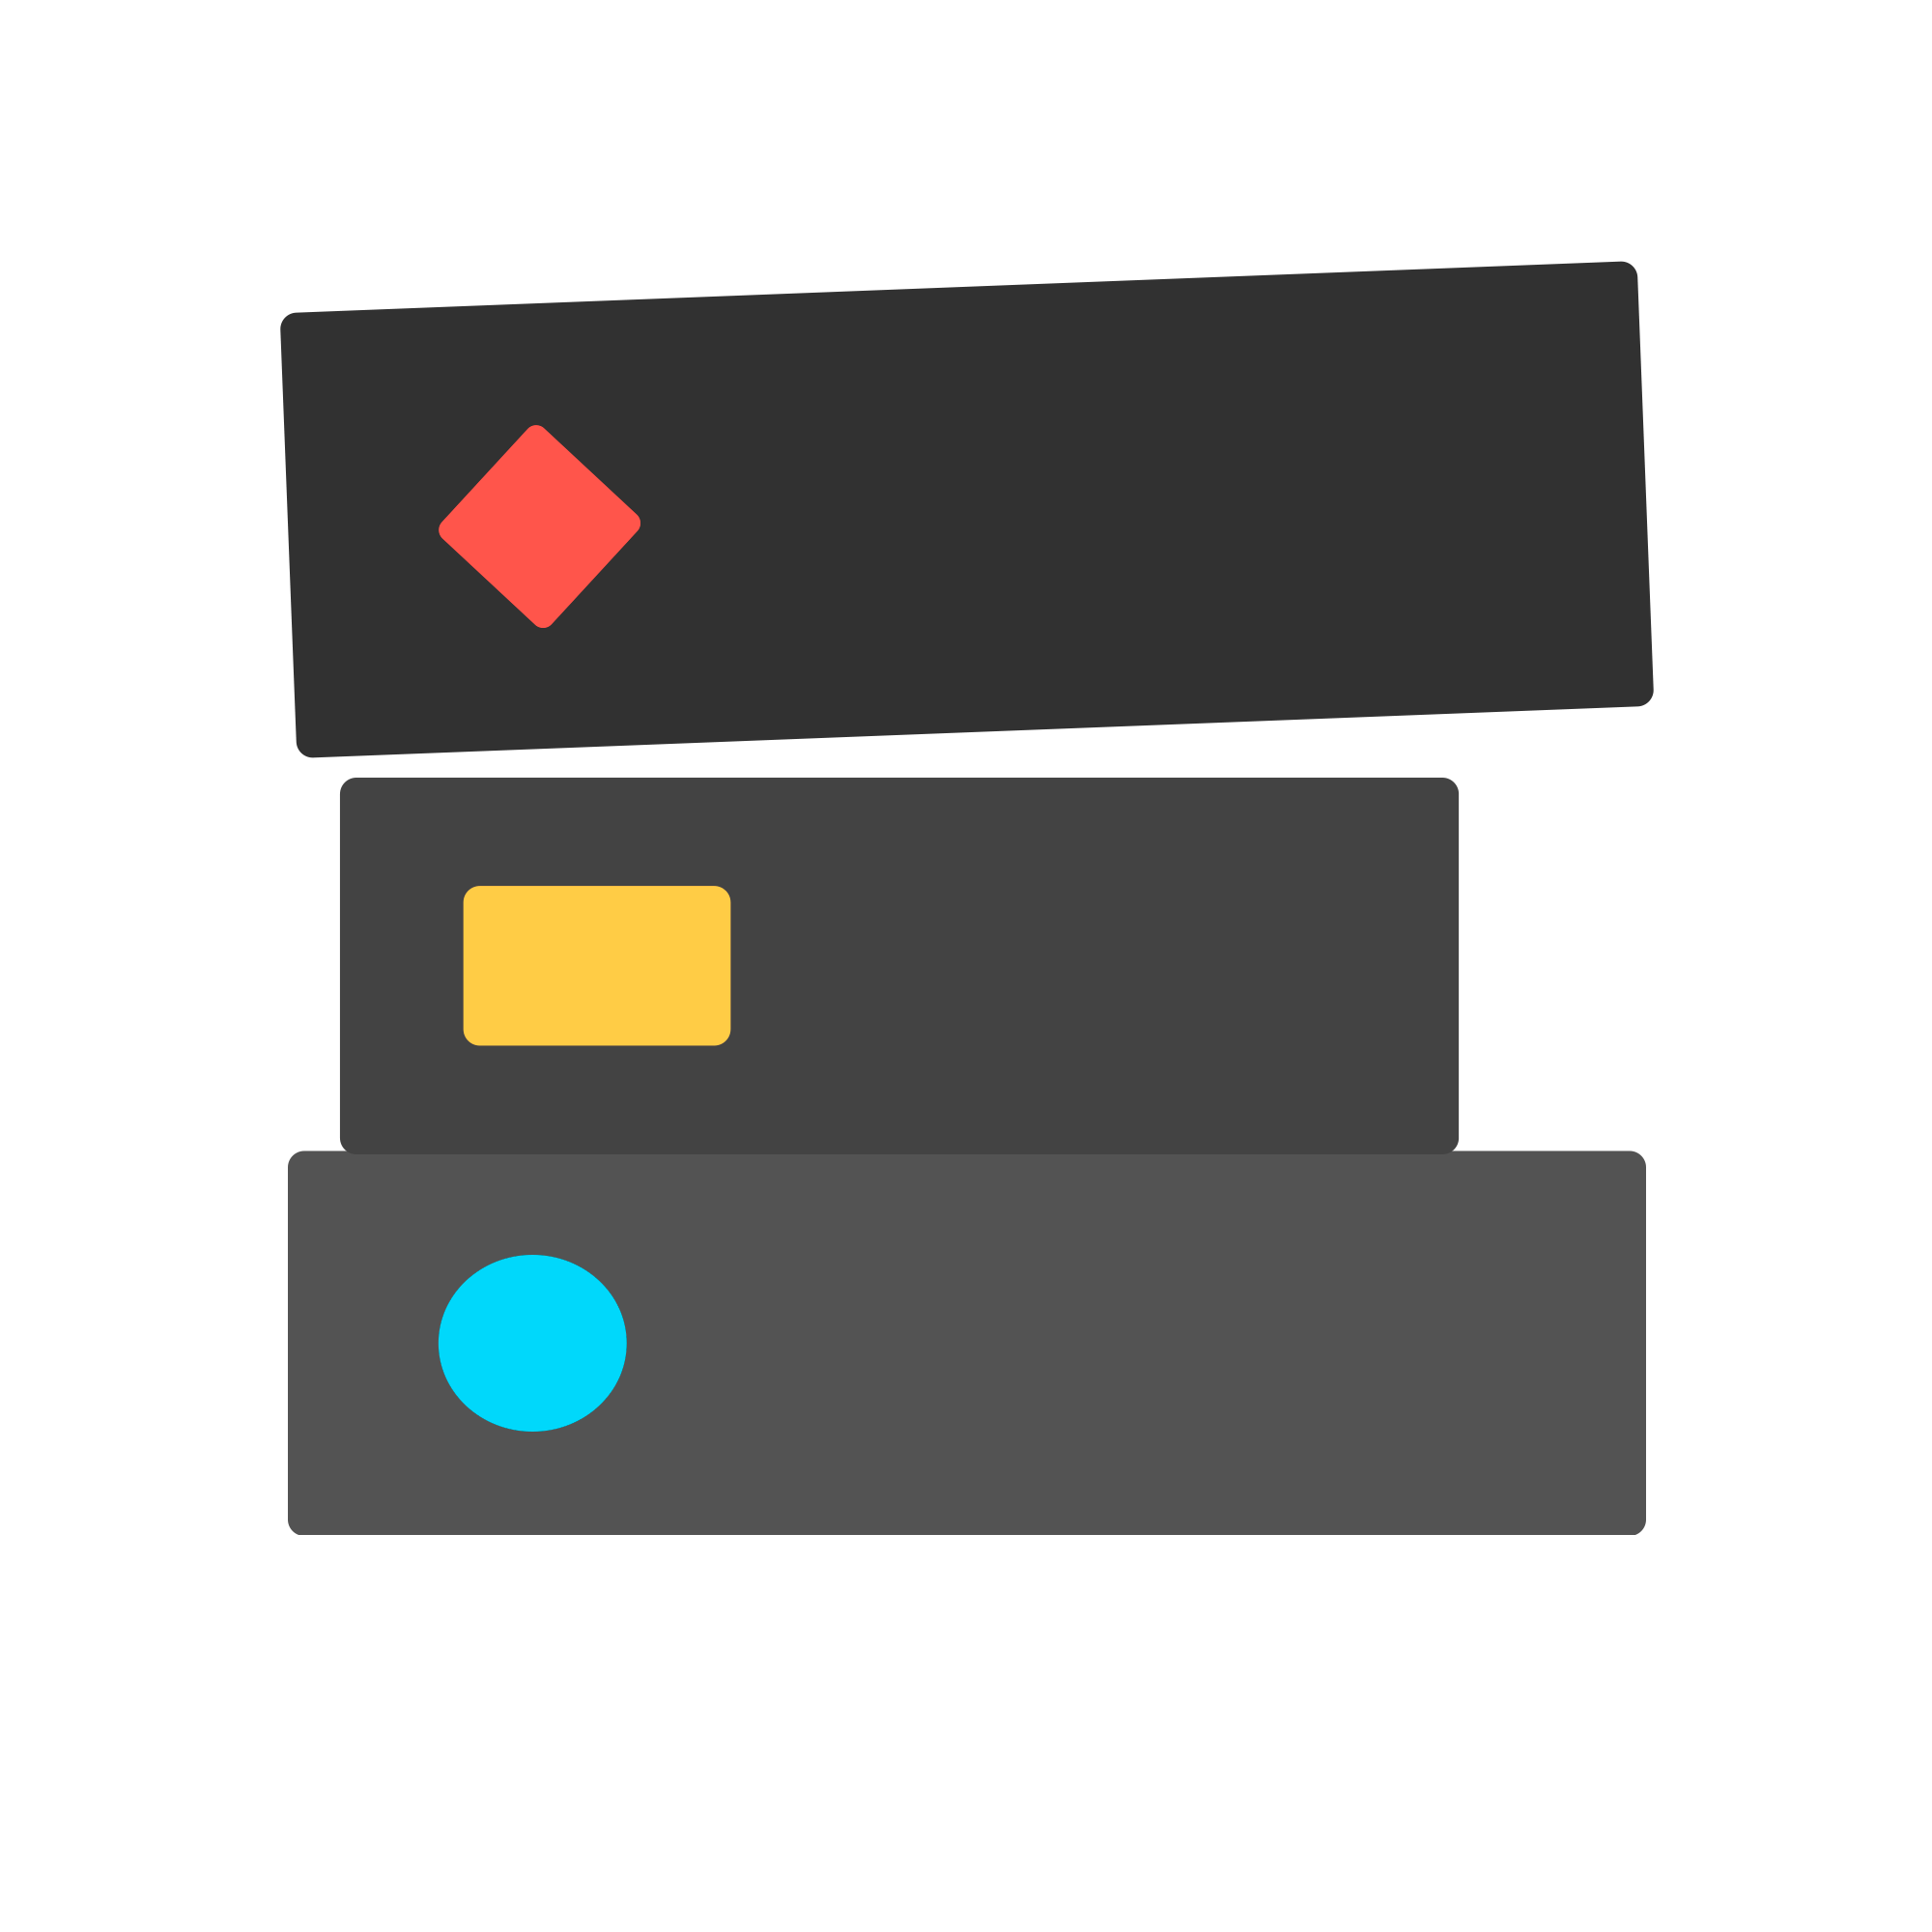
\includegraphics[width=0.5\textwidth]{img/DBCase_logo.png}
\end{figure}
%%
\section{Introducción}
DBCASE 2.0 surge como una actualización al proyecto DBCASE con la que se pretende dar un nuevo aspecto al diseño de la interfaz de usuario y continuar con la implementación de nuevas funcionalidades.\\

El programa está destinado principalmente al uso académico y por ello ha sido pensado como una herramienta didáctica que ayude al alumno en su proceso de aprendizaje, aunque también puede ser usada profesionalmente como una manera fácil y rápida de construir una base de datos relacional. Por ello la herramienta permite al usuario crear una base de datos funcional a partir de un diagrama sin necesidad de que conozca ningún lenguaje de programación de base de datos, lo que es perfecto para alumnos que se estén iniciando en la materia.\\

La herramienta está desarrollada íntegramente utilizado el lenguaje de programación Java.

%%
\subsection{Antecedentes}
El proyecto DBCase 2.0 es la continuación de dos proyectos anteriores.\\

\textbf{DBDT} de sistemas informáticos (2007/2008)\\
Autores del proyecto:
\begin{itemize}
    \item Alberto Milán Gutierrez.
    \item Miguel Martinez Segura
    \item Francisco Javier Cáceres González
    \item Profesora Directora: Yolanda García Ruiz
\end{itemize}

\textbf{DBCase} de sistemas informáticos (2008/2009)\\
Autores del proyecto:
\begin{itemize}
    \item Rodrigo Denis Cepeda Mateos
    \item Cristina Marco de Francisco
    \item Tello Serrano Gordillo
\end{itemize}
El proyecto servía como una herramienta bastante útil, pero que debido al paso de los años había quedado algo obsoleta. Sobre todo en lo que respecta a su interfaz gráfica.
%%
\subsection{Objetivos}
El principal objetivo del proyecto era rehabilitar la aplicación para su uso académico en las aulas, para lo cual era necesario satisfacer dos cuestiones.
\begin{itemize}
    \item Actualizar el diseño de la interfaz gráfica de la aplicación, haciéndola más usable y moderna.
    \item Corregir los posibles errores que arrastrase la aplicación desde versiones anteriores y continuar añadiendo funcionalidades nuevas.
\end{itemize}

    \chapter{Estudio de soluciones existentes}
Durante la primera fase de este proyecto se realizó una investigación y análisis de herramientas disponibles en el mercado que tuvieran características y funcionalidades similares a las que ofrece DBCase.\\

En este proceso de estudio se han investigado herramientas que permiten la realización de diagramas entidad relación, analizando las mecánicas que ofrecen para la creación de los mismos.\\

También se han investigado herramientas que permitieran la traducción de un esquema conceptual a un código ejecutable por un gestor de base de datos, analizando el flujo de trabajo llevado a cabo por la herramienta.
\section{Draw.io}

Draw.io \cite{drawio} es una aplicación web de código abierto que permite realizar de manera sencilla todo tipo de diagramas siendo una de las herramientas más usadas a nivel mundial para este cometido.\\

Draw.io proporciona una gran cantidad de distintos elementos y formas que pueden ser usadas en el diagrama y proporciona una gran versatilidad y capacidad de personalización sin dejar de ser una herramienta muy intuitiva.\\

Con respecto al proyecto DBCase la herramienta ofrece soluciones muy interesantes en cuanto a la fase de diseño del diagrama entidad relación.\\

\begin{itemize}
    \item Dispone de una barra lateral de elementos y una barra superior de herramientas, mostrando al usuario todos los elementos disponibles así como todas las acciones realizables por el usuario en un solo vistazo.
    \item Permite guardar y abrir proyectos, tanto desde el sistema de ficheros como desde otros sistemas de almacenamientos en la nube.
    \item Permite tener varios proyectos abiertos al mismo tiempo.
    \item El establecimiento de conexiones entre elementos se puede realizar de forma gráfica.
    \item Ofrece la posibilidad de cambiar el tema de la interfaz.
\end{itemize}
\section{Smart Draw}
Smart Draw \cite{smartdraw} es una herramienta de software privativo que permite realizar múltiples tipos de diagrama. Cuenta con una versión web y otra de escritorio para los principales sistemas operativos. Está enfocada principalmente en diagramas de ingeniería y arquitectura y cuenta con un módulo específico para la creación de diagramas entidad relación muy completo.\\

En cuanto al espacio de trabajo que proporciona es muy similar al ofrecido por la herramienta Draw.io (posee una barra lateral de elementos y otra superior de herramientas, permite guardar y abrir proyectos y trabajar con varios al mismo tiempo).\\

Otro punto a destacar es la facilidad de conectar y crear elementos en el diagrama. Llevando el cursor al borde de un elemento permite crear otro idéntico directamente conectado. De esta forma se simplifica enormemente el proceso de conexión de elementos. Esta función es interesante y podría extrapolarse para añadir nuevas entidades a una relación. Esta funcionalidad es complementaria a la de establecer conexiones de forma gráfica, que también ofrece Draw.io.
\section{EDRPLus}
EDRPlus \cite{edrplus} es una aplicación web de uso gratuito, que está específicamente diseñada para la creación de diagramas de bases de datos. La herramienta da la opción de crear diagramas entidad relación y esquemas relacionales. Además la aplicación permite traducir el diagrama entidad relación directamente a código sql.\\

La herramienta permite guardar proyectos y, mediante el inicio de sesión subir y acceder a tus proyectos guardados en el servidor, sacando un gran provecho al hecho de ser una aplicación web.\\

Como vemos, la herramienta permite realizar las dos funcionalidades principales que pretende DBCase.\\

\begin{enumerate}
    \item En cuanto al espacio de trabajo proporcionado para el diseño del diagrama entidad relación, la herramienta es, en general menos potente e intuitiva que las vistas anteriormente. La creación de elementos y conexiones se realiza mediante un panel superior en el que aparecen todos los elementos disponibles (atributos, entidades, relaciones y etiquetas), y todas las acciones disponibles (establecer una conexión, seleccionar, eliminar, deshacer y rehacer) en una sola fila de botones de texto, lo que resulta confuso.\\
    
    Al tener un elemento seleccionado aparece un panel de opciones en la parte derecha de la pantalla que permite modificar todas las opciones del mismo (nombre, tipo, cardinalidad en el caso de relaciones etc). Esto parece una buena solución aunque puede dar pie a que se queden elementos sin modificar, ya que en ningún momento obliga al usuario ni siquiera a establecer un nombre para el elemento.
    
    \item La herramienta no comprueba en ningún momento la corrección del diagrama. Puedes crear atributos sueltos o entidades débiles sin entidad fuerte, en este sentido es menos potente de lo que ya ofrece DBCase.\\
    
    \item La herramienta no ofrece la opción de generar el modelo relacional.
    
    \item Para generar el código SQL, el usuario debe salir del panel de edición e ir al listado de sus documentos, solo desde ahí y mediante un menú desplegable se da la posibilidad de generarlo, lo cual resulta muy poco intuitivo.
    \item No dispone de atajos de teclado.
\end{enumerate}
\section{SqlDBM}
\section{Conclusiones del estudio}
    \chapter{Resultados y conclusiones}
%%
\section{Resultados}
DBCASE permite realizar el proceso de diseño y creación de una base de datos de forma sencilla mediante una interfaz de escritorio, centrándose en ayudar al estudiante en su proceso de aprendizaje.\\

%%%%%%%%%
\subsection*{Espacio de trabajo}
El usuario puede modificar muchos aspectos del espacio de trabajo para hacer más cómoda su experiencia con la aplicación.\\

Puede escoger el idioma, el tema y la perspectiva que desee. También puede redimensionar los paneles para adaptarlos a sus necesidades.
\begin{figure}[H]
    \centering
    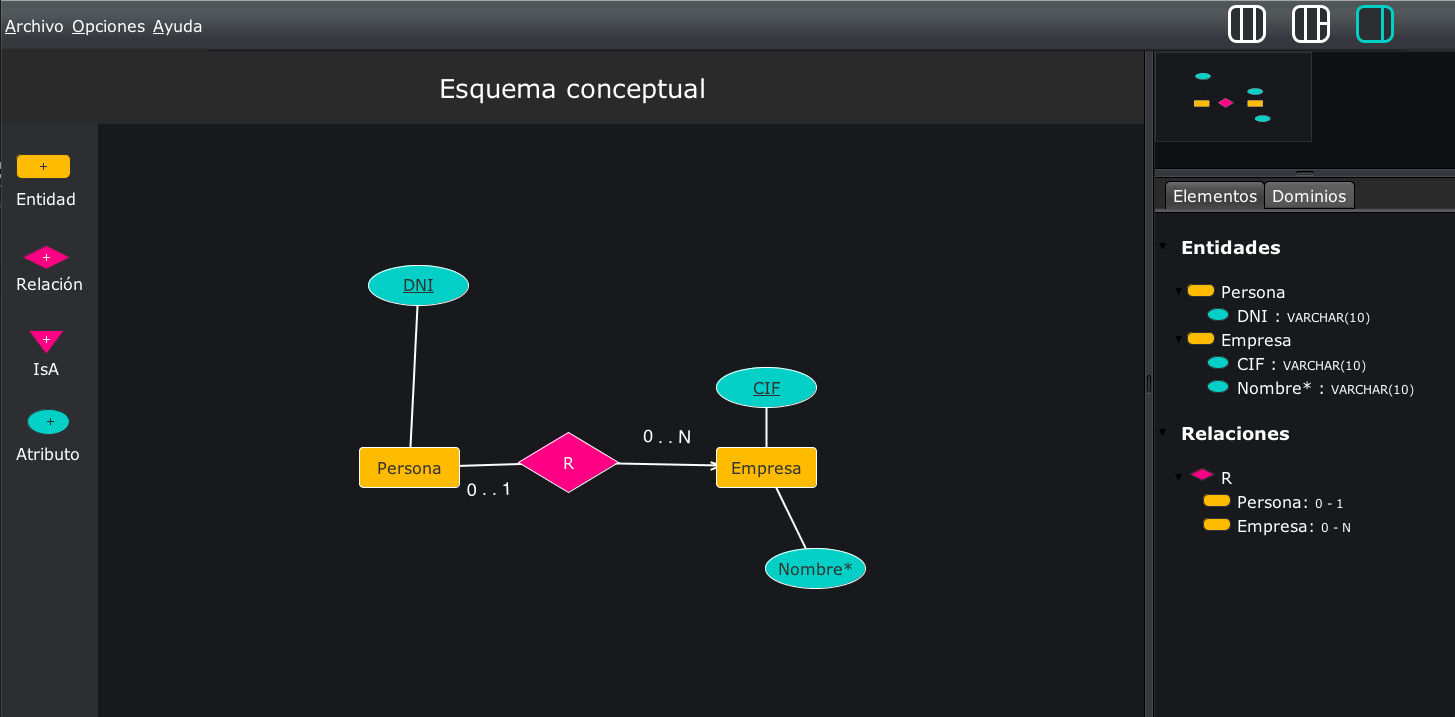
\includegraphics[width=1\textwidth]{img/black.png}
    \caption{Ejemplo de espacio de trabajo personalizado}
\end{figure}

%%%%%%%%%
\subsection*{Creación de un diagrama}
El primer paso es la creación y el diseño de un diagrama entidad relación. Para ello se debe seleccionar una de las dos perspectivas que muestran el panel de diseño.\\

Para añadir elementos al diagrama el usuario dispone de dos opciones.
\begin{itemize}
    \item Haciendo clic derecho sobre el panel de diseño. Se mostrará un menú desplegable que permite insertar cualquier tipo de elemento.
    \item Utilizando la barra lateral, pulsando en los iconos que representan los elementos.
\end{itemize}
A la hora de insertar elementos, se pueden escoger mediante distintos cuadros de diálogo las características de los mismos. Por ejemplo en el caso de insertar una nueva entidad se debe indicar el nombre, y se da la opción de que la entidad sea débil con respecto a otra existente en el diagrama. En tal caso se debe seleccionar esa entidad fuerte y dar nombre a la relación que las une.\\

El procedimiento para eliminar elementos del diagrama es el siguiente:
\begin{itemize}
    \item primero se debe seleccionar un elemento o un conjunto de elementos (bien abarcando todos los elementos con el ratón o bien seleccionando de uno en uno y manteniendo pulsada la tecla shift).
    \item Tras realizar la selección se puede eliminar los elementos de dos formas:
    \begin{itemize}
        \item Hacer clic derecho sobre el elemento, tras lo cual se mostrará un menú desplegable, en el que una de las opciones es la de eliminar el elemento.
        \item Pulsando la tecla de suprimir.
    \end{itemize}
    Antes de finalizar el proceso se mostrará un cuadro de confirmación.
\end{itemize}

%%%%%%%%%
\subsection*{Relaciones}
Uno de los elementos básicos en los diagramas entidad relación son las relaciones entre entidades.\\

Para conectar una relación con una entidad el usuario debe hacer clic derecho sobre la relación y pulsar en la opción \enquote{añadir una entidad} del menú desplegable. Tras ello se abrirá un cuadro de diálogo en el que se debe seleccionar la entidad y elegir con qué cardinalidad se desea establecer el vínculo. También se da la posibilidad de indicar un nombre para el rol del enlace.

%%%%%%%%%
\subsection*{Restricciones}
El usuario puede añadir restricciones a cualquier elemento del diagrama. Estas restricciones serán importantes a la hora de crear el script sql que genere la base de datos.\\

Para insertar restricciones a los elementos el usuario debe pulsar clic derecho sobre un elemento del diagrama y pulsar \enquote{restricciones} dentro del menú desplegable.\\

Tras ello se abrirá un cuadro de diálogo que permite al usuario crear una lista con las restricciones para ese elemento.

%%%%%%%%%
\subsection*{Dominios}
Al crear un atributo el usuario debe indicar qué dominio está vinculado con ese atributo. Aunque en un diagrama entidad relación no es necesaria esta información, sí que es importante a la hora de generar el esquema físico ya que todas las columnas de una tabla deben tener un dominio.\\

El programa ofrece por defecto once de los dominios más comúnmente usados pero también da la posibilidad al usuario de crear su propios dominios.
\begin{itemize}
    \item Pulsando clic derecho sobre un espacio vacío en el diagrama y pulsando en la opción \enquote{crear dominio}.
    \item Seleccionando la pestaña de dominios y haciendo clic en el botón de \enquote{nuevo}.
\end{itemize}
Tras ello se abre un cuadro de diálogo en el que el usuario debe indicar el nombre del dominio, el tipo base, y los valores que puede adoptar separados por comas.
%%%%%%%%%
\subsection*{Generación de códigos}
El siguiente paso tras el diseño del diagrama entidad relación es la generación de los esquemas lógico o físico.\\

Para ello el usuario debe pulsar en los botones de generar dispuestos en ambos paneles. De existir errores o advertencias, los paneles informarán de forma clara de qué se trata.\\

Una vez generados los códigos, el usuario tiene la opción de editarlos para añadir, modificar o eliminar cualquier cuestión. Una vez el usuario esté satisfecho con el código, tiene la posibilidad de exportarlo a un archivo en formato texto, o también en formato sql en el caso del esquema físico.\\

El programa también da la posibilidad de ejecutar el esquema físico directamente en el gestor de base de datos que haya seleccionado.
%%
\section{Discusión y conclusiones}%[SPA-ENG]
\textit{[ESP]}\\
La aplicación ha mejorado enormemente el aspecto gráfico y se ha adaptado en la medida de lo posible a los estándares de diseño de hoy en día. Una de las limitaciones que se ha sufrido es la de arrastrar las librerías de Jung \cite{jung} y la implementación de la interfaz mediante java swing. Hubiese sido muy interesante haber creado una nueva interfaz usando las opciones que proporciona java FX.\\

También hubiese sido interesante generar el diagrama usando otra librería distinta a Jung, ya que durante todos estos años han surgido mejores soluciones para la creación de este tipo de diagramas.\\

Al tratarse de un proyecto individual y al ser el principal objetivo hacer que la aplicación volviese a ser usable se decidió centrar los esfuerzos en ello, manteniendo por tanto las librerías de la anterior versión.\\

También se ha mejorado la funcionalidad de la aplicación corrigiendo errores, mejorando sobre todo el esquema lógico y añadiendo nuevas funcionalidades a la aplicación.\\

En lo personal, el proyecto me ha permitido aprender en profundidad cómo es el desarrollo de una aplicación de escritorio, así como aumentar mis conocimientos sobre el lenguaje java y sobre la programación orientada a objetos. Especialmente he aprendido a como construir una interfaz de usuario completa y funcional.\\

\textit{[ENG]}\\

The application has greatly improved the graphic user interface and adapted as far as possible to the design standards of today. One of the limitations that has been suffered is having to use the Jung \cite{jung} and java swing libraries. It would have been interesting to have created a new interface using the options provided by Java FX.\\

It would also have been interesting to generate the diagram using another library other than Jung, since during all these years better solutions for the creation of such diagrams have emerged.\\

Being an individual project and being the main objective to make the application usable again, it was decided to focus efforts on it, thus maintaining the libraries of the previous version.\\

The functionality of the application has also been improved by correcting errors, especially improving the logical schema and adding new functionalities to the application.\\

Personally, the project has allowed me to learn in depth how is the development of a desktop application, as well as increase my knowledge about java language and object-oriented programming. I especially learned how to build a complete and functional user interface.\\


    \chapter{Resultados y conclusiones}
%%
\section{Resultados}
DBCASE permite realizar el proceso de diseño y creación de una base de datos de forma sencilla mediante una interfaz de escritorio, centrándose en ayudar al estudiante en su proceso de aprendizaje.\\

%%%%%%%%%
\subsection*{Espacio de trabajo}
El usuario puede modificar muchos aspectos del espacio de trabajo para hacer más cómoda su experiencia con la aplicación.\\

Puede escoger el idioma, el tema y la perspectiva que desee. También puede redimensionar los paneles para adaptarlos a sus necesidades.
\begin{figure}[H]
    \centering
    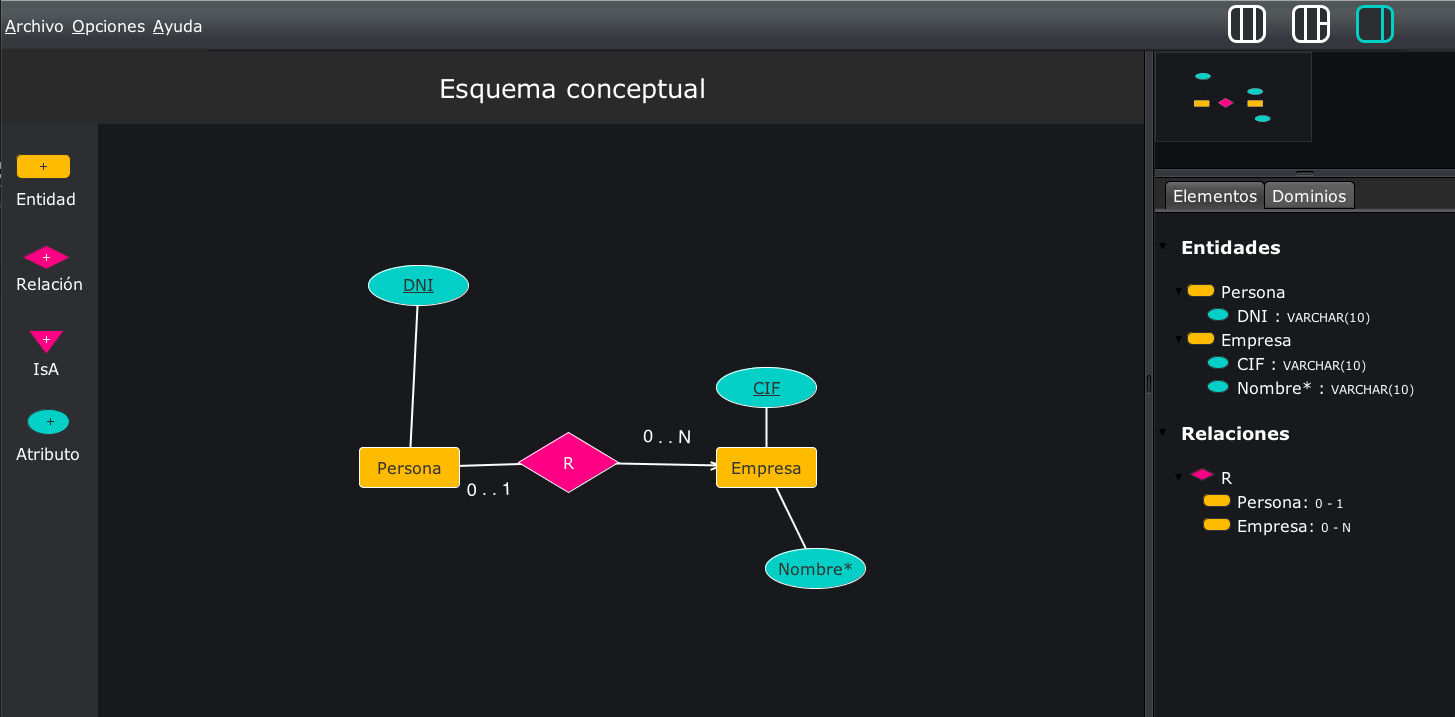
\includegraphics[width=1\textwidth]{img/black.png}
    \caption{Ejemplo de espacio de trabajo personalizado}
\end{figure}

%%%%%%%%%
\subsection*{Creación de un diagrama}
El primer paso es la creación y el diseño de un diagrama entidad relación. Para ello se debe seleccionar una de las dos perspectivas que muestran el panel de diseño.\\

Para añadir elementos al diagrama el usuario dispone de dos opciones.
\begin{itemize}
    \item Haciendo clic derecho sobre el panel de diseño. Se mostrará un menú desplegable que permite insertar cualquier tipo de elemento.
    \item Utilizando la barra lateral, pulsando en los iconos que representan los elementos.
\end{itemize}
A la hora de insertar elementos, se pueden escoger mediante distintos cuadros de diálogo las características de los mismos. Por ejemplo en el caso de insertar una nueva entidad se debe indicar el nombre, y se da la opción de que la entidad sea débil con respecto a otra existente en el diagrama. En tal caso se debe seleccionar esa entidad fuerte y dar nombre a la relación que las une.\\

El procedimiento para eliminar elementos del diagrama es el siguiente:
\begin{itemize}
    \item primero se debe seleccionar un elemento o un conjunto de elementos (bien abarcando todos los elementos con el ratón o bien seleccionando de uno en uno y manteniendo pulsada la tecla shift).
    \item Tras realizar la selección se puede eliminar los elementos de dos formas:
    \begin{itemize}
        \item Hacer clic derecho sobre el elemento, tras lo cual se mostrará un menú desplegable, en el que una de las opciones es la de eliminar el elemento.
        \item Pulsando la tecla de suprimir.
    \end{itemize}
    Antes de finalizar el proceso se mostrará un cuadro de confirmación.
\end{itemize}

%%%%%%%%%
\subsection*{Relaciones}
Uno de los elementos básicos en los diagramas entidad relación son las relaciones entre entidades.\\

Para conectar una relación con una entidad el usuario debe hacer clic derecho sobre la relación y pulsar en la opción \enquote{añadir una entidad} del menú desplegable. Tras ello se abrirá un cuadro de diálogo en el que se debe seleccionar la entidad y elegir con qué cardinalidad se desea establecer el vínculo. También se da la posibilidad de indicar un nombre para el rol del enlace.

%%%%%%%%%
\subsection*{Restricciones}
El usuario puede añadir restricciones a cualquier elemento del diagrama. Estas restricciones serán importantes a la hora de crear el script sql que genere la base de datos.\\

Para insertar restricciones a los elementos el usuario debe pulsar clic derecho sobre un elemento del diagrama y pulsar \enquote{restricciones} dentro del menú desplegable.\\

Tras ello se abrirá un cuadro de diálogo que permite al usuario crear una lista con las restricciones para ese elemento.

%%%%%%%%%
\subsection*{Dominios}
Al crear un atributo el usuario debe indicar qué dominio está vinculado con ese atributo. Aunque en un diagrama entidad relación no es necesaria esta información, sí que es importante a la hora de generar el esquema físico ya que todas las columnas de una tabla deben tener un dominio.\\

El programa ofrece por defecto once de los dominios más comúnmente usados pero también da la posibilidad al usuario de crear su propios dominios.
\begin{itemize}
    \item Pulsando clic derecho sobre un espacio vacío en el diagrama y pulsando en la opción \enquote{crear dominio}.
    \item Seleccionando la pestaña de dominios y haciendo clic en el botón de \enquote{nuevo}.
\end{itemize}
Tras ello se abre un cuadro de diálogo en el que el usuario debe indicar el nombre del dominio, el tipo base, y los valores que puede adoptar separados por comas.
%%%%%%%%%
\subsection*{Generación de códigos}
El siguiente paso tras el diseño del diagrama entidad relación es la generación de los esquemas lógico o físico.\\

Para ello el usuario debe pulsar en los botones de generar dispuestos en ambos paneles. De existir errores o advertencias, los paneles informarán de forma clara de qué se trata.\\

Una vez generados los códigos, el usuario tiene la opción de editarlos para añadir, modificar o eliminar cualquier cuestión. Una vez el usuario esté satisfecho con el código, tiene la posibilidad de exportarlo a un archivo en formato texto, o también en formato sql en el caso del esquema físico.\\

El programa también da la posibilidad de ejecutar el esquema físico directamente en el gestor de base de datos que haya seleccionado.
%%
\section{Discusión y conclusiones}%[SPA-ENG]
\textit{[ESP]}\\
La aplicación ha mejorado enormemente el aspecto gráfico y se ha adaptado en la medida de lo posible a los estándares de diseño de hoy en día. Una de las limitaciones que se ha sufrido es la de arrastrar las librerías de Jung \cite{jung} y la implementación de la interfaz mediante java swing. Hubiese sido muy interesante haber creado una nueva interfaz usando las opciones que proporciona java FX.\\

También hubiese sido interesante generar el diagrama usando otra librería distinta a Jung, ya que durante todos estos años han surgido mejores soluciones para la creación de este tipo de diagramas.\\

Al tratarse de un proyecto individual y al ser el principal objetivo hacer que la aplicación volviese a ser usable se decidió centrar los esfuerzos en ello, manteniendo por tanto las librerías de la anterior versión.\\

También se ha mejorado la funcionalidad de la aplicación corrigiendo errores, mejorando sobre todo el esquema lógico y añadiendo nuevas funcionalidades a la aplicación.\\

En lo personal, el proyecto me ha permitido aprender en profundidad cómo es el desarrollo de una aplicación de escritorio, así como aumentar mis conocimientos sobre el lenguaje java y sobre la programación orientada a objetos. Especialmente he aprendido a como construir una interfaz de usuario completa y funcional.\\

\textit{[ENG]}\\

The application has greatly improved the graphic user interface and adapted as far as possible to the design standards of today. One of the limitations that has been suffered is having to use the Jung \cite{jung} and java swing libraries. It would have been interesting to have created a new interface using the options provided by Java FX.\\

It would also have been interesting to generate the diagram using another library other than Jung, since during all these years better solutions for the creation of such diagrams have emerged.\\

Being an individual project and being the main objective to make the application usable again, it was decided to focus efforts on it, thus maintaining the libraries of the previous version.\\

The functionality of the application has also been improved by correcting errors, especially improving the logical schema and adding new functionalities to the application.\\

Personally, the project has allowed me to learn in depth how is the development of a desktop application, as well as increase my knowledge about java language and object-oriented programming. I especially learned how to build a complete and functional user interface.\\


    
    \begin{thebibliography}{9}
\subsubsection*{Comentario.}
\section*{Sectio1}
%%%%%%%%%%%%%%%%%%%%%%%%%%%%%%%%%%%%%%
\bibitem{nimbus} 
Nimbus Look and Feel
\\\url{https://docs.oracle.com/javase/tutorial/uiswing/lookandfeel/nimbus.html}
%%%%%%%%%%%%%%%%%%%%%%%%%%%%%%%%%%%%%%
\bibitem{json} 
Json
\\\url{https://es.wikipedia.org/wiki/JSON}
%%%%%%%%%%%%%%%%%%%%%%%%%%%%%%%%%%%%%%
\bibitem{singleton} 
Singleton
\\\url{https://es.wikipedia.org/wiki/Singleton}
%%%%%%%%%%%%%%%%%%%%%%%%%%%%%%%%%%%%%%
\bibitem{g2d} 
Graphics2D
\\\url{https://docs.oracle.com/javase/7/docs/api/java/awt/Graphics2D.html}
\end{thebibliography}
    \newpage
\chapter*{Sobre \teflon}
\noindent
\textsc{Teflon(cc0 1.0(documentación) MIT(código))%\cite{dPaciosTeflon}% 
es una plantilla de \LaTeX\phantom{} creada por David Pacios Izquierdo con fecha de Enero de 2018. Con atribuciones de uso CC0.}\\\\
\noindent
Esta plantilla fue desarrollada para facilitar la creación de documentación profesional para Trabajos de Fin de Grado o Trabajos de Fin de Máster. La versión usada es la 1.3.\\\\
\noindent
V:\textsc{1.3 Overleaf V2 with pdfLaTeX, margin 1in, NO-bib}
\vfill
\noindent
\textsc{\textbf{\underline{Contacto}}\\ \textbf{Autor:} David Pacios Izquiero \\ \textbf{Correo:} \url{dpacios@ucm.es}\\ \textbf{ASCII:} \url{asciifdi@gmail.com}\\ Despacho 110 - Facultad de Informática}
\end{document}
%%%%%%%%%%%%%%%%%%%%%%%%%%%%%%%%%%%%%%%%%%%%%%%%%%%%%%%%%%%%%%%%%%%